\begin{figure}
  \centering
  \begin{tikzpicture}
    \draw[very thick, ->] (0,0) -- (3.8,0) node[anchor=north] {x};
    \draw[very thick, ->] (0,0) -- (0,3.3) node[anchor=east] {y};
    \node at (-0.2,0) {0};
    \node at (0,-0.2) {0};
    % first system
    \draw[red, local bounding box=S1, thick]
      (1.2,0.2) rectangle (3.7,2.7);
    \node[red]
      at ({$(S1.west)!0.37!(S1.east)$} |- {$(S1.south)!0.12!(S1.north)$})
      {\small System 2};
    % second system
    \draw[blue, local bounding box=S2, thick]
      (0.2,1.2) rectangle (3.2,3.2);
    \node[blue]
      at ({$(S2.west)!0.31!(S2.east)$} |- {$(S2.south)!0.85!(S2.north)$})
      {\small System 1};
  \end{tikzpicture}
  \hspace{30pt}
  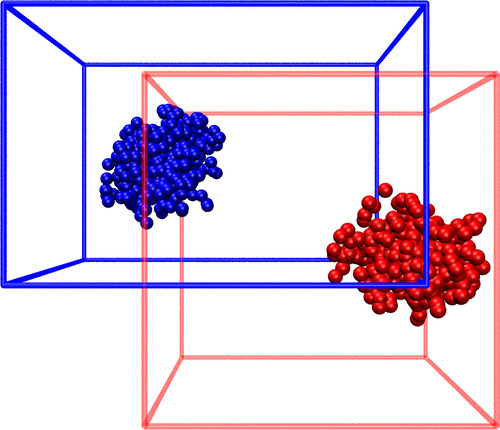
\includegraphics[scale=0.6]{JoinSystems-fig_a.jpg}
  \caption{
    Original systems offset via lower box bounds in the respective files in
    \tt{Examples/JoinSystems} folder (\tt{System1.lammpstrj} and
    \tt{System2.lammpstrj} files).
  }
\end{figure}
